\documentclass{article}

\usepackage{tikz}
\begin{document}

%\def\input_layer{1}
%\def\hidden_layer_0{5}

\def\hdist{2}

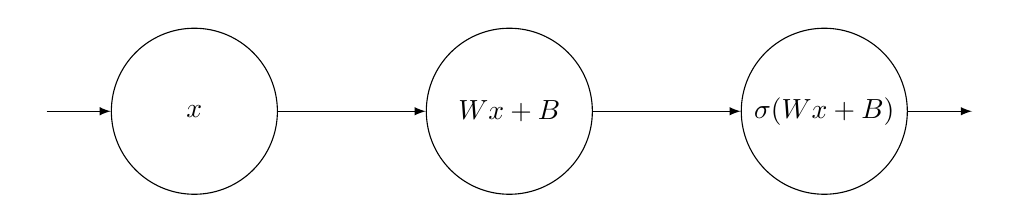
\begin{tikzpicture}


\node (left_input) at (-2, 0) {};
\node[draw, circle, minimum size=60pt] (input) at (0, 0) {$x$};
\draw[->,>=latex] (left_input) -- (input);



% plot the second layer
\node[draw,circle, minimum size=60pt] (output) at (4,0) {$Wx+B$};
\draw[->, >=latex] (input) -- (output);


%plot sigmoid
\node[draw , circle , minimum size=60pt] (sigmoid) at (8,0) {$\sigma(Wx+B)$};
\draw[->, >=latex] (output) -- (sigmoid);

\node (outter) at (10,0) {};
\draw[->, >=latex] (sigmoid) -- (outter);



%
%
%
%\node (input) at (-2,0) {} ;
%\node[draw, circle] (n00) at (0,0) {$x_{0,0}$};
%
%\foreach \i in {0,...,\hidden_layer_0}
%  \node[draw, circle] ({\i}) at (2,2*\i)  {};
%  
%\draw[->] (1) -- (2);
%
%\node[draw, circle] (n10) at (4,4) {$x_{1,0}$};
%
%\draw[->, >=latex] (input) -- (n00);
%
%\draw[->,>=latex] (n00) -- (n10);


\end{tikzpicture}



\end{document}